\documentclass[10pt, conference, compsocconf]{IEEEtran}

\usepackage{url}
\usepackage{graphicx}

% correct bad hyphenation here
\hyphenation{op-tical net-works semi-conduc-tor}


\begin{document}

\title{Design and Prototype Implementation of the WattsApp Telemetry Platform}
\author{
\IEEEauthorblockN{Vaibhav Bajpai, Vitali Bashko, Catalin David, Siarhei Kuryla, Vladislav Perelman, Johannes Schauer, \\Nikolay Melnikov, Anuj Sehgal, J\"{u}rgen Sch\"{o}nw\"{a}lder\\}
\IEEEauthorblockA{Computer Science, Jacobs University Bremen, Campus Ring 1, 28759 Bremen, Germany
\\\{v.bajpai, v.bashko, c.david, s.kuryla, v.perelman, j.schauer, \\n.melnikov,
s.anuj, j.schoenwaelder\}@jacobs-university.de}
}

\maketitle

\begin{abstract}
Telemetry is an important function of the Internet of Things as it
is being developed and deployed today. Of particular interest within
this area are energy monitoring services. In this paper we describe
WattsApp, a social telemetry gathering and comparison platform, which
was built as a demonstrator that integrates technologies from embedded
systems to mobile applications. We used the SNMP protocol stack developed
for the Contiki embedded operating system to retrieve telemetry information
from a hardware interface that reads data from S0 meters (e.g., power
meters, fluid meters). A web interface and an Android mobile application
lets users view this data. To ensure privacy of users' data, it is
only stored at users' own premises and all communication takes place
over encrypted connections. This paper provides an overview of the
implementation of WattsApp. 
\end{abstract}

\section{Introduction}

The emergence of embedded computing devices capable of wireless communications
is leading to the emergence of an Internet of Things (IoT). The availability
of network computing devices capable of performing limited tasks themselves
opens up opportunities to develop multiple new applications in various
fields. From home automation to an energy balanced smart grid for
electricity generation and distribution, the IoT is expected to introduce
a plethora of new computing services that rely on integrating existing
software services on the Internet with the control and data-gathering
capabilities of embedded devices.

However, since most embedded devices to be used in the IoT do not
use an IEEE 802.11 WiFi interface \cite{durvy08making}, interconnecting
them with the existing Internet infrastructure requires the development
of protocols and systems that take into account the low-power and
lossy radio standards currently used in embedded wireless sensor networks.
To avoid the emergence of devices that are neither interoperable nor documented, the IETF developed the 6LoWPAN standard \cite{rfc-4,rfc-5} to enable IPv6 networking over the IEEE 802.15.4 radio standard, which is commonly used in embedded networks \cite{6lowpan-1}.

Using IoT technologies, like 6LoWPAN, and integrating them with well
established Internet and mobile application services, WattsApp was
built as a technology demonstrator to showcase a typical application
of the IoT. Development was completed within a short time-frame of
approximately one month within the framework of a graduate networking
lab course. The WattsApp telemetry platform integrates embedded hardware
with standard network management protocols, like SNMP, and allows
users to view telemetry (e.g. energy, water or gas consumption) and
share it using the Facebook social network. Multicast-DNS (mDNS) provides
for automatic discovery of services (meters and data-collectors) offered
within a network.

\begin{figure}[t]
\begin{centering}
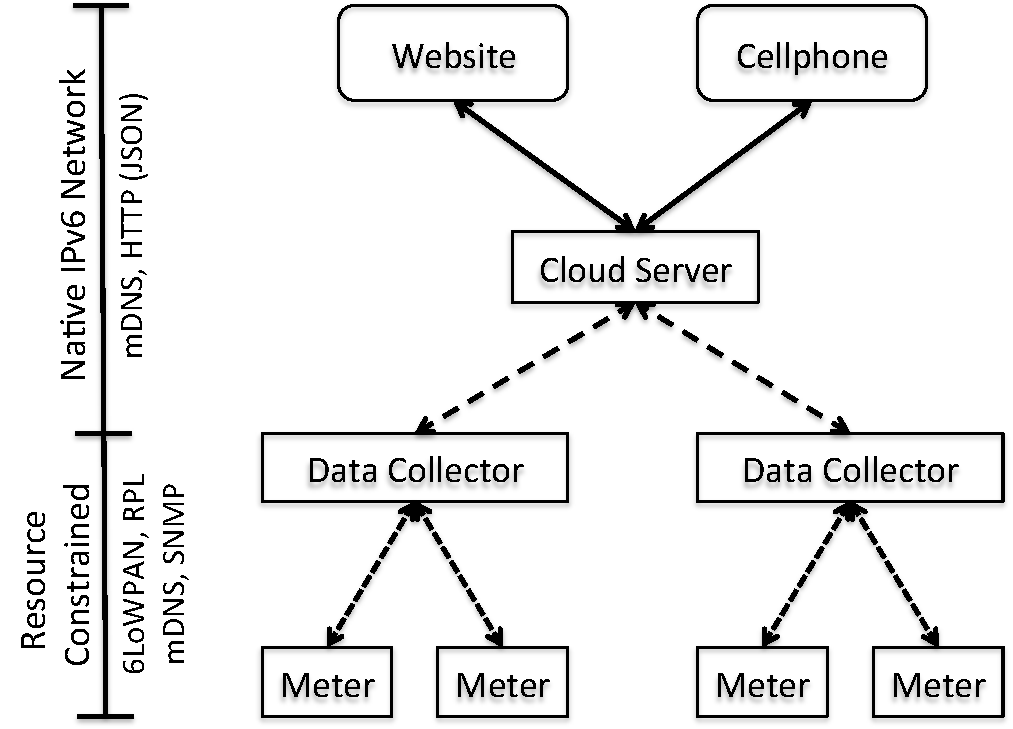
\includegraphics[scale=0.4]{images/wattsapp-overview} 
\par\end{centering}

\caption{An overview of the WattsApp architecture. The meters and data collectors
typically function within a resource constrained network, whereas
all other components are based in traditional IP networks.\label{fig:wattsapp}}
\end{figure}


The following sections of this paper present an overview on the design
of WattsApp along with a short discussion on related work. Starting
from the architecture described in Section 2, we discuss the hardware
interface (Section 3), the polling and storage components (Section
4), the gatekeeper located on the cloud server (Section 5) and the
user interfaces (Section 6). Related work is discussed in Section
7, before we conclude the paper.


\section{Architecture and Application Overview}

The WattsApp telemetry platform is designed to collect and report
time-series data from different sources. Data such as power consumption
can be collected using embedded sensors or external meters attached
to IPv6 enabled sensor boards.

An overview of the WattsApp architecture can be seen in Figure \ref{fig:wattsapp}.
Our implementation integrates a native IPv6 network with an 802.15.4
resource constrained network. Within the resource constrained network,
meters measure power consumption. Each meter uses the Contiki operating
system \cite{contiki-2} running on an Atmel AVR Raven platform and
has the ENTITY-MIB \cite{rfc4133} and ENTITY-SENSOR-MIB \cite{rfc3433}
implemented within the Contiki SNMP agent \cite{aims-snmp-contiki}.
These meters are able to interface with different data reporting devices
using appropriate hardware interfaces. We designed an electricity
consumption meter based on the S0-Interface \cite{iec62053-31}, however,
the versatility of the S0-interface makes it easy to make hardware
interfaces for water or gas consumption as well. In our setup, the
data collectors deployed at users' premises to retrieve the data collected
from the S0-interface circuit using SNMP.

The data collector communicates with the WattsApp server, i.e. the
gatekeeper located at the cloud server (in Figure \ref{fig:wattsapp})
using encrypted RESTful HTTP requests using the JSON data format.
The cloud server is used for authentication and access control. It
also acts as an intermediary between front-end clients and the data
collectors/meters. A website and an Android OS mobile application
are the front-ends which retrieve and display metered data using requests
to the cloud server.

The aim of developing WattsApp was to demonstrate the integration
of multiple Internet technologies, from native IPv6 and resource constrained
networks to mobile and web-based applications, into a single system
by using pre-existing tools. Specifically, the demonstrator was designed
as a student project for the Advanced Distributed Systems Lab%
\footnote{http://cnds.eecs.jacobs-university.de/courses/adsl-2011/%
} graduate course within a period of about one-and-half months. Given
more time, the system could likely have been designed to provide better
performance, however, by using mostly pre-existing tools it became
clear that it is possible to rapidly develop a stable IPv6 capable
system.

Furthermore, since each meter device is capable of being assigned
a globally routable IPv6 address, it can be reasoned that any device,
mobile or otherwise, could directly communicate with them. Reusing
protocols such as SNMP for management and monitoring of these devices
then presents a great advantage because a number of existing tools
(e.g. graphing tools like Cacti) can be used without adaptation.


\section{Hardware Interface}

Since WattsApp is a telemetry platform, gathering data is one of the
most important tasks. Since the IoT is expected to be an enabling
technology for smart-grids, designing meters capable of measuring
energy, water and gas consumption was deemed important for the demonstrator.
Not only was it necessary to build the hardware to gather this information,
but ensuring that this information could be accessed in an Internet
standards compliant way was also important.

\begin{figure*}[t]
\begin{centering}
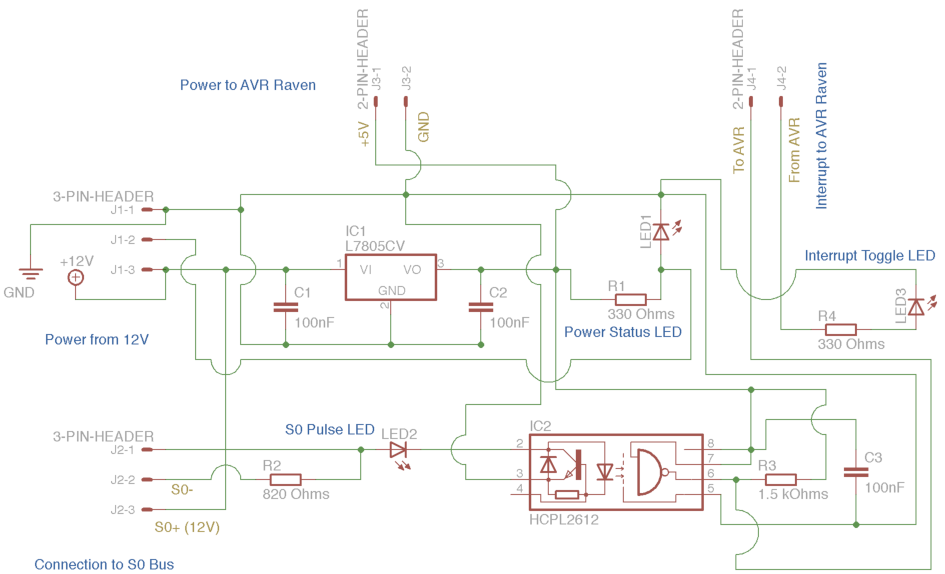
\includegraphics[scale=.75]{images/schematic} 
\par\end{centering}

\caption{A circuit diagram showing the S0-interface circuit that converts S0
current pulses to digital voltage pulses. The HCPL2612 digital optocoupler
is used to isolate the high voltage and current circuit from the digital
part. When the S0 circuit causes a high current pulse, the HCPL2612
allows a 5V circuit to be completed, thereby causing a voltage pulse
that can be counted. The L7805CV voltage regulator is used to ensure
a clean and stable 5V digital signal.}


\label{fig:S0-interface} 
\end{figure*}


The following sub-sections present the design of the metering hardware,
along with information on the interface that allows retrieval of this
data over SNMP.


\subsection{S0 Pulse Counter Circuit}

High power AC-current circuits and digital circuits normally do not
mix very well due to the high differences in the voltage and currents
involved in such systems. As such, in order to measure electricity
consumption, with the ability to transfer this information into digital
systems poses some challenges. Furthermore, since the aim of WattsApp
was not only to monitor electricity consumption, but also other utilities
like water and gas, it was important to choose a metering method that
enables recording consumption values for all these utilities.

The S0-interface was chosen for this purpose since there are many
meters capable of measuring electricity, gas and water consumption
based on this system. The S0-interface is a pulse-modulation system
that, unlike digital systems, is based on current rather than voltage
modulation. An S0 meter takes in a DC voltage between 12-27V as power
supply and causes the current across the output lines to rise up between
10-27mA, once a cumulative load of a certain value is achieved. For
example, the S0 electricity meter we use causes a current pulse between
10-27mA once 1 kWh of energy has been consumed.

While counting these current pulses gives us a method of calculating
the amount of energy consumed over a certain time period, digital
systems are not capable of directly measuring current, and as a consequence
current pulses. Digital systems normally work by equating 5V to a
digital 1 (on) and 0V to a digital 0 (off). As such, pulse-modulation
in digital systems normally works by measuring a voltage of 5V as
on and 0V as off. This necessitates a method of converting the S0
current pulses to digital voltage pulses. We achieved this conversion
by building an interface circuit, the schematic for which can be seen
in Figure \ref{fig:S0-interface}.

Since the S0 meters operate at voltages between 12-27V it is important
to ensure that this voltage does not leak into the digital part of
the circuit, which operates at 5V. As such, we use a digital optocoupler
device which takes the output from the S0 meter. Each time the S0
meter outputs an ON pulse of 10-27mA current, an LED within the optocoupler
turns on and allows for the digital circuit to turn on as well. Not
only does this ensure that higher voltages are never leaked into the
5V digital circuit, but it also converts a current pulse into a digital
voltage pulse. These digital voltage pulses may now be counted and
aggregated to obtain consumption values over time.


\subsection{AVR Raven Contiki SNMP Interface}

\label{subsec:avr-contiki-snmp}

Once the output from the S0 meters is available in digital form, this
must be aggregated and a method provided for it to be retrieved via
a network. Since the aim was to integrate everything using IPv6, this
retrieval must happen using Internet standard technologies and the
meters must be reachable via IPv6. To accomplish this, the AVR Raven
hardware platform was chosen since it is capable of running the Contiki
OS, which brings IPv6 networking to embedded devices. Furthermore,
since a SNMP agent is available for Contiki, the telemetry can be
retrieved using an implementation of the ENTITY-MIB and ENTITY-SENSOR-MIB.

To retrieve consumption values from the S0-interface circuit, described
in the previous sub-section, the output of the interface circuit was
connected to a digital-input line on the AVR Raven. A driver for the
AVR platform, which caught an interrupt each time a voltage of 5V
was observed on the connected digital-input line, was written. This
made it easy to count energy consumption since each time the interrupt
occurred, in case of our meter it meant that 1 kWh of energy had been
consumed. This data is aggregated by the AVR Raven and can be retrieved
using SNMP. A poller script, described in greater detail in following
sections, running on data-collectors retrieves this data and stores
it in a SQLite database.

It is important to note that the stability of this system has been
excellent. Ever since the system went online in late October, the
only downtime that was encountered was when the coffee-machine being
monitored was removed for cleaning, prompting the University cleaning-crew
to also disconnect our meter. However, this was also quickly recovered
from since reconnecting the system was not difficult. An overview
of the complete metering solution can be seen in Figure \ref{fig:meter-overview}.


\section{Polling and Storing}

Since the meters integrated with WattsApp can provide telemetry in
many different units and formats, the polling script is responsible
for making any device specific adaptations before storing the data
in the database. This data is then relayed to the clients by a collector
service, via a gatekeeper running as web-service on the cloud server.
This section provides an insight into the poller and collector services
of WattsApp.


\subsection{The Polling Script}

The poller is responsible for collecting data from the IPv6-enabled
meters in order to store it into a database. Since interfacing to
devices often requires device specific adaptations, we decided to
write the polling engine in the Python language. While Python in general
is a perfect fit for these kind of tasks, we were surprised that we
could not find a single packaged SNMP extension for Python that supported
IPv6 well.

As such, we ended up using a wrapper around the NET-SNMP tools in
order to fetch data. Furthermore, we learned quickly that the poller
needs to be resilient to all sorts of failures. In particular, we
occasionally experience 802.15.4 failures exceeding the retransmissions
we do. Furthermore, data storage can fail, in particular during times
of development or software updates. The originally rather short script
did grow into a script defining a class \texttt{Snmp} wrapping the
NET-SNMP \texttt{snmpget} command, a class \texttt{Meter} modeling
a single meter (e.g., a temperature meter or an energy meter), and
a class \texttt{Exporter} modeling an exporter providing access to
several meters.

A discovery method detects meters at startup and assigns UUIDs to
them as needed. The script is capable of detecting discontinuities
and taking appropriate actions. During the development phase, Python's
flexible logging API helped a lot since it allowed us to get notified
about failures via Email, something invaluable since many problems
occur at unforeseen times of the day. There are still many improvements
possible put perhaps it is also time to consider the adoption of
polling engines of applications like Nagios%
\footnote{\url{http://www.nagios.org}%
} or Cacti%
\footnote{\url{http://www.cacti.net/}%
} that already incorporate many more advanced features.


\subsection{The Collector}

\begin{figure}[t]
\begin{centering}
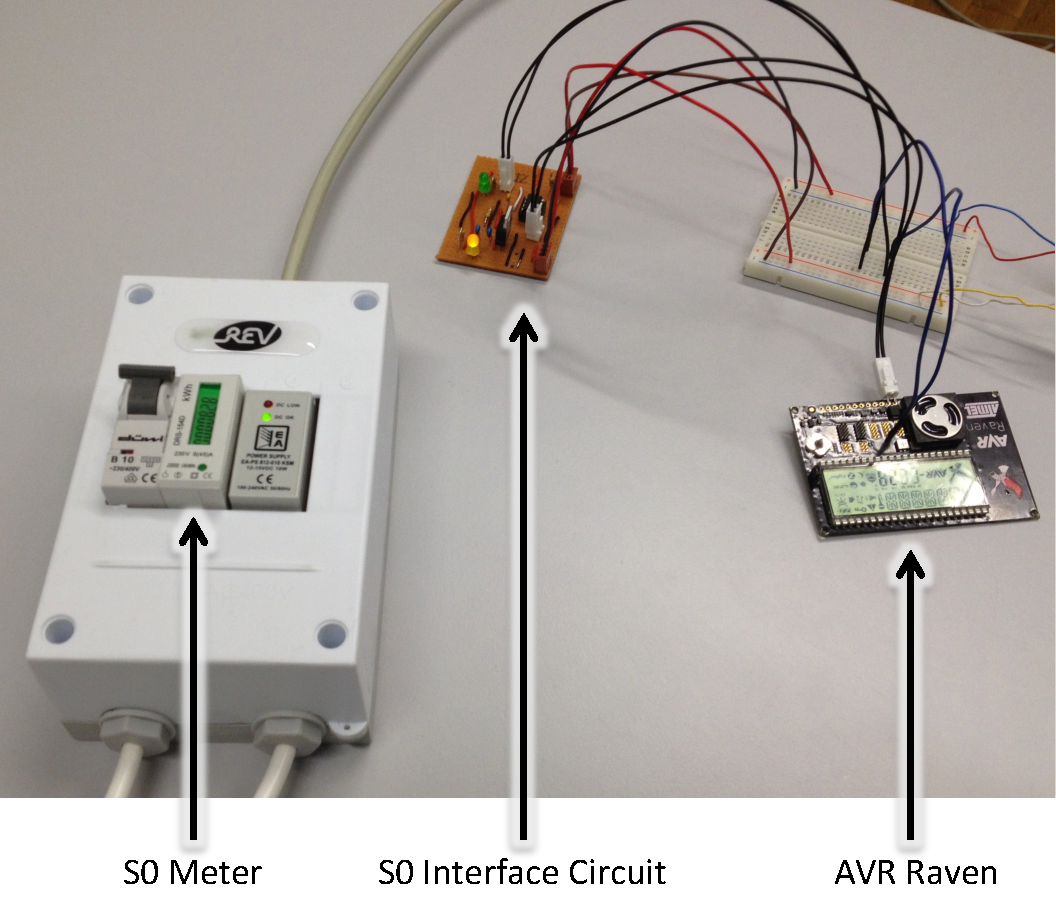
\includegraphics[scale=0.4]{images/s0-meter} 
\par\end{centering}

\caption{The S0 interface for the electricity meter along with the AVR Raven
based data exporting device. The S0 interface converts the S0 current
pulses into digital voltage pulses, which are logged via interrupts
in the AVR Raven in order to count energy consumption and export this
data to a collector via a poller script.\label{fig:meter-overview}}
\end{figure}

The WattsApp Collector was chosen to be written in Node.js \cite{nodejs:2010},
which is an event driven, asynchronous I/O JavaScript environment
based on Google's libv8 JavaScript engine. This choice was made, since
the event-driven nature of Node.js allowed concurrent processing of
requests without the drawbacks of adding complexity that comes with
a multithreaded approach.

The WattsApp Collector allows clients to query for meter data via
HTTP. It advertises its service upon startup via an mDNS advertisement
so that any clients in the local network can discover the collector
and retrieve data from it, if they are authorized to do so. All data
transfer between the collector and clients is encrypted using the
built-in Node.js TLS library and authentication of clients is done
using X.509 certificates. If an unauthorized client tries to connect
to the WattsApp Collector or a connection without TLS is initiated,
an error message is returned to the initiator.

After successful authentication, a client can send HTTP GET requests
to the collector and receive data in JSON format. If a valid query
is received by the collector, it responds with the appropriate JSON
message by retrieving data from the SQLite database into which the
poller writes data collected from the meters. Functionality exposed
by the Collector to authorized clients includes listing of all meters,
showing meter details, blacklisting and renaming meters and setting
the physical location of meters. The GET query allows the client to
specify the meter for which data should be returned along with the
time interval that data is requested for.

Collectors are located within a users' premises since this is the
data aggregation point. Not only does this encourage data privacy,
since it is not located in a central location, but also limits the
chances of unauthorized access since only clients for which the user
installs a X.509 certificate are permitted to communicate with it.


\section{The Gatekeeper - Cloud Server}

\begin{figure}[t]
\begin{centering}
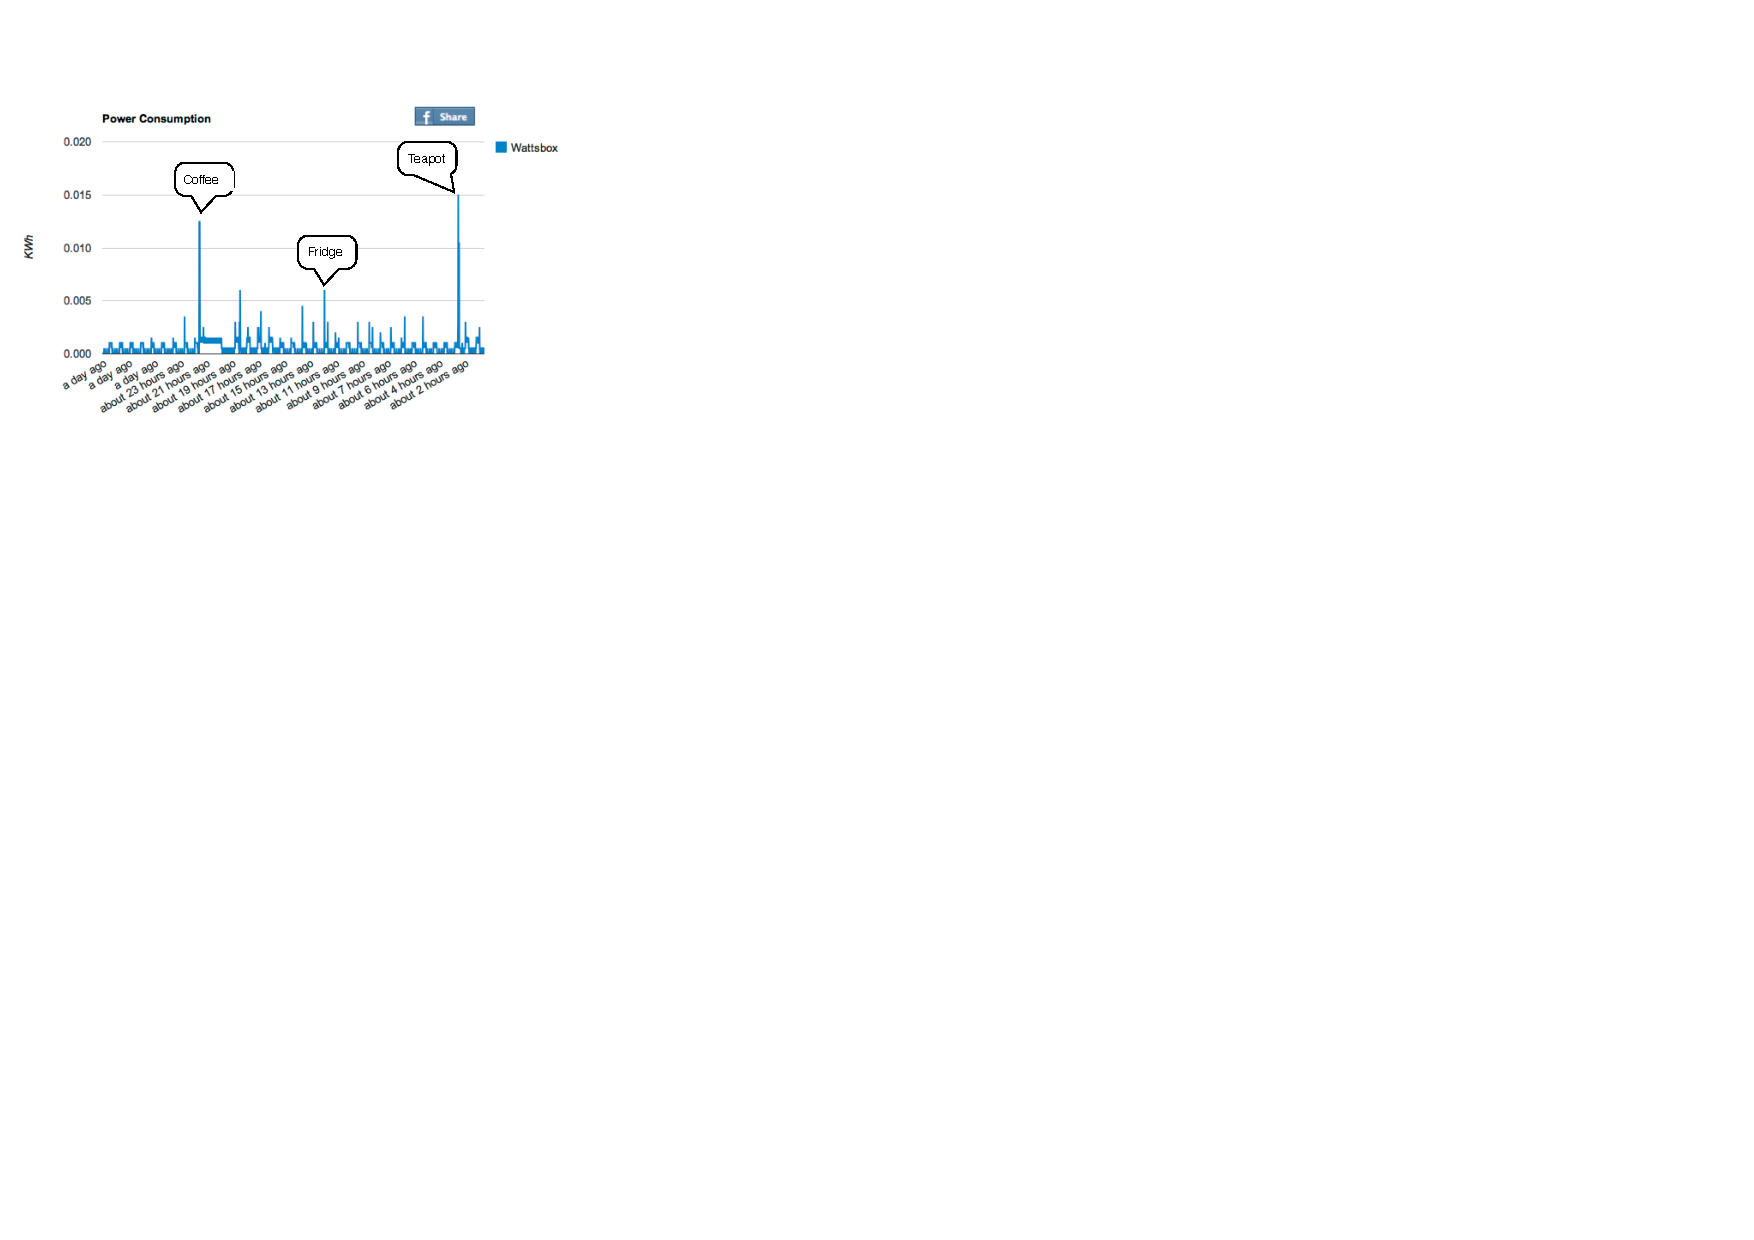
\includegraphics[scale=0.93]{images/power-consumption} 
\par\end{centering}

\caption{A typical graph output on the website client interface. This graph
plots the power consumption obtained from a single meter connected
to an exporter named Wattsbox. Annotations can be added to these graphs
and it can also be shared on Facebook. }


\label{fig:website-power-consumption}
\end{figure}

The gatekeeper web service, which resides on the cloud server (as
in Figure \ref{fig:wattsapp}) performs the function of authenticating
users and performing access control to data from collectors. This
service is written in PHP using the Vanilla MVC Framework. Once a
user is successfully authenticated by using the Facebook single-sign-on,
it provides both the user interfaces (web and android) application
with meter data through a RESTful interface. To perform the authentication,
the user interfaces provide the gatekeeper with the token and email
address that Facebook returns to the application once an authentication,
directly with Facebook, is completed. The gatekeeper then uses this
token to check with Facebook whether the email address supplied with
the token matches the user requesting access and what permission levels
are associated with that user, i.e. which meters the user has access
to and whether these can be edited as an administrator.

The meter data can be filtered and requested along a particular time
frame. The queries to rename or change the location of a meter from
either of the interfaces are also managed through the gatekeeper.
The gatekeeper in itself, for privacy reasons, does not store any
data which it passes to the user interfaces, but is meant to keep
the user authentication and authorization centralized and simplistic.
All data exchanges between the user interfaces and the gatekeeper
web-service take place using the JSON data format.

\section{User Interfaces}

The visualization and interaction of the meter readings is possible
either using our standalone website or through a freely available
Android application. The web application serves two purposes; firstly,
it is meant to provide a lowest common denominator for all users and
to be the most powerful platform to deliver the richest experience
in energy usage visualization. On the other hand, the mobile application
is meant to provide data to users on the move.


\subsection{Web Application}

\begin{figure}[t]
\begin{centering}
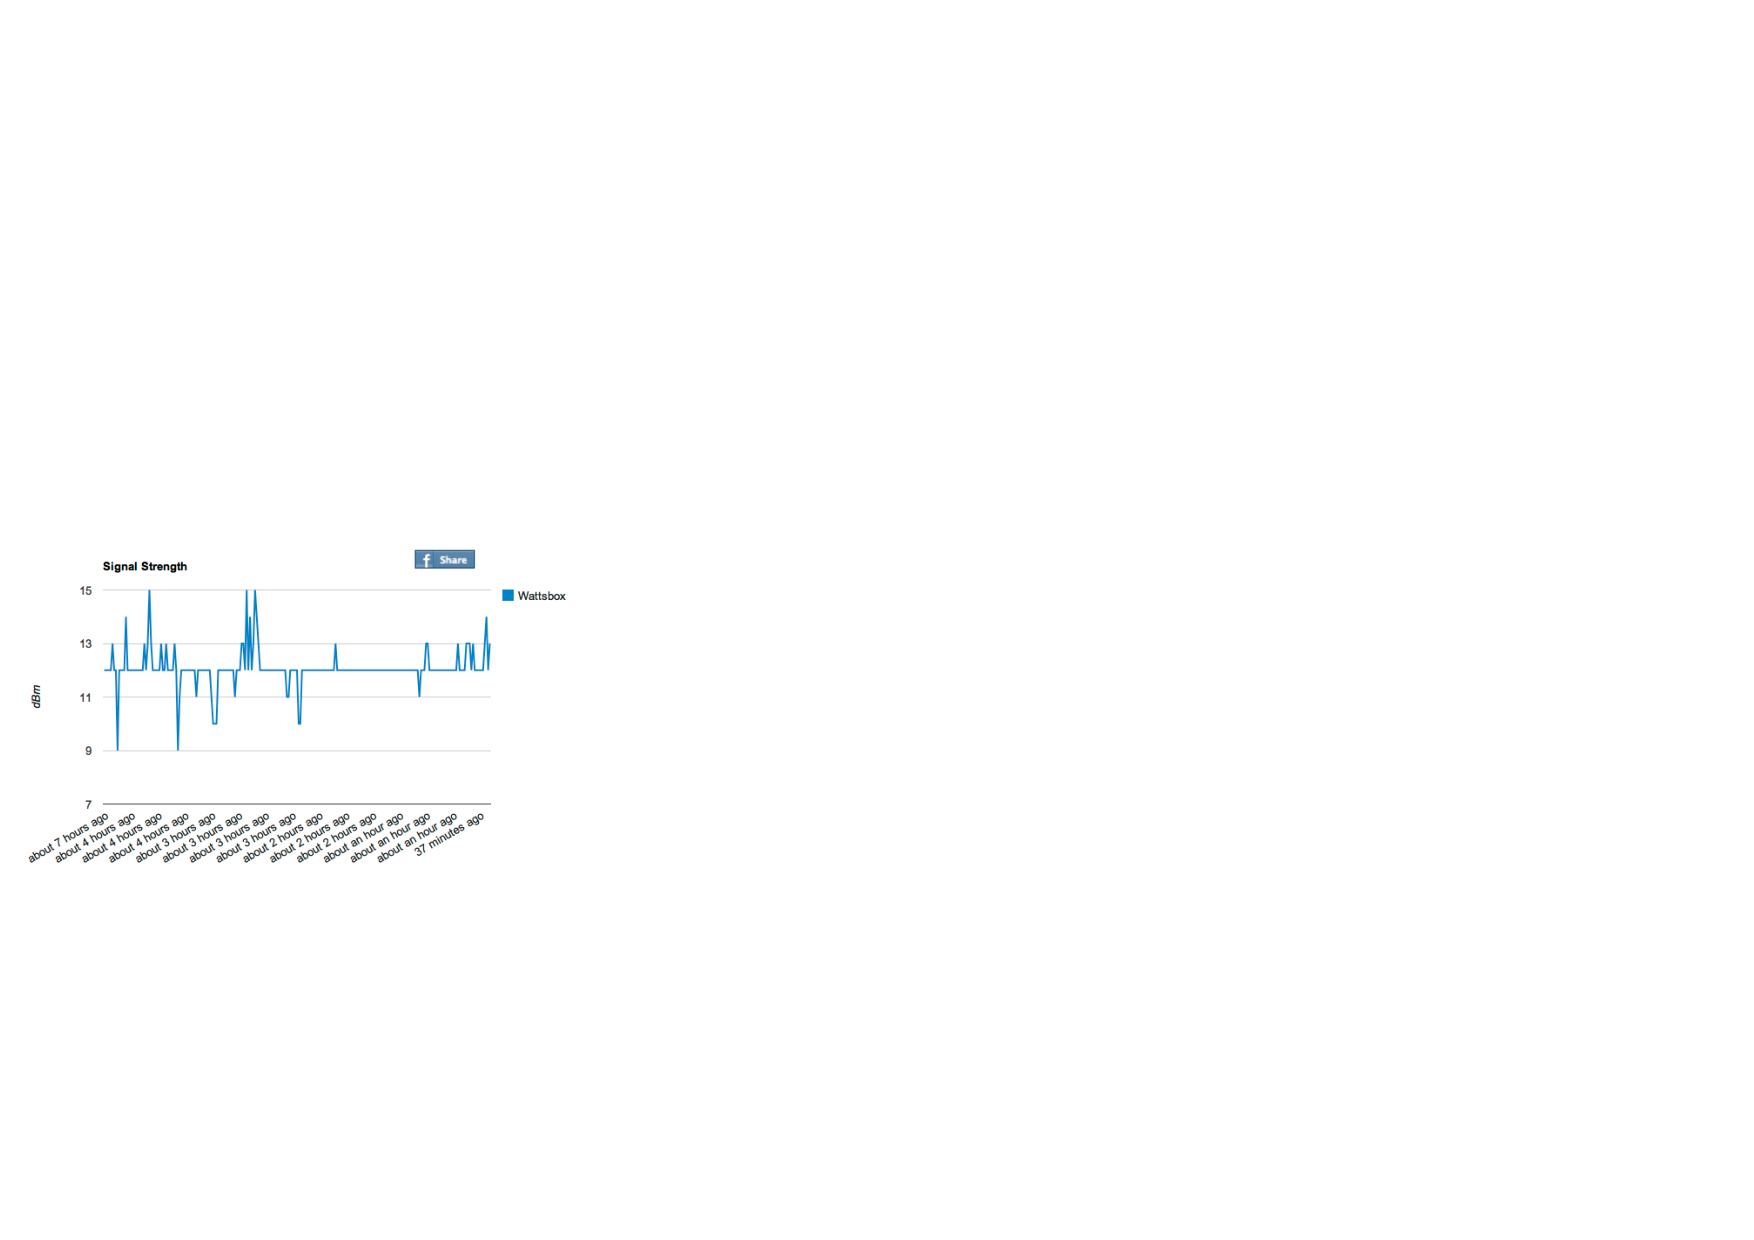
\includegraphics[scale=0.93]{images/signal-strength} 
\par\end{centering}

\caption{A typical graph output on the website client interface. Instead of
energy consumption this graph plots the radio signal strength of the
connection to an exporter named Wattsbox. Annotations can be added
to these graphs and it can also be shared on Facebook. }


\label{fig:website-signal-strength}
\end{figure}

The web application%
\footnote{http://www.wattsapp.net%
} provides a simple platform for a user to view the usage of the energy
meters. The web application uses Facebook's Javascript SDK %
\footnote{https://developers.facebook.com/docs/reference/javascript/%
} to provide single sign-on using OAuth 2.0 \cite{oauth}. Once logged
in, the user can view the list of the collectors he can administer
or has been given permission to view the data from. A similar layout
is available for the list of meters as well.

The collectors and their associated meters have their locations pinned
on a google map using the Google Maps API. The energy usage can be
visualized using either tree maps or line charts. Tree maps can be
used to relatively compare and contrast the energy usage of the meters,
which provide data in the directly comparable units. This display
is similar to the one found in our Android application, as shown in
Figure \ref{fig:treemap-android}. A thorough analysis of the energy
usage of a particular meter is also possible. For instance, the graph
in Figure \ref{fig:website-power-consumption} shows the visualization
of our energy meter that measures the power consumption of the fridge
and the coffee machine connected in our office. Similarly, the signal
strength of the AVR Raven that exports this energy usage is shown
in Figure \ref{fig:website-signal-strength}. The website is built
using the jQuery framework \cite{Bibeault:2008:JA:1407181}.


\subsection{Android Application}

\begin{figure}[t]
\begin{centering}
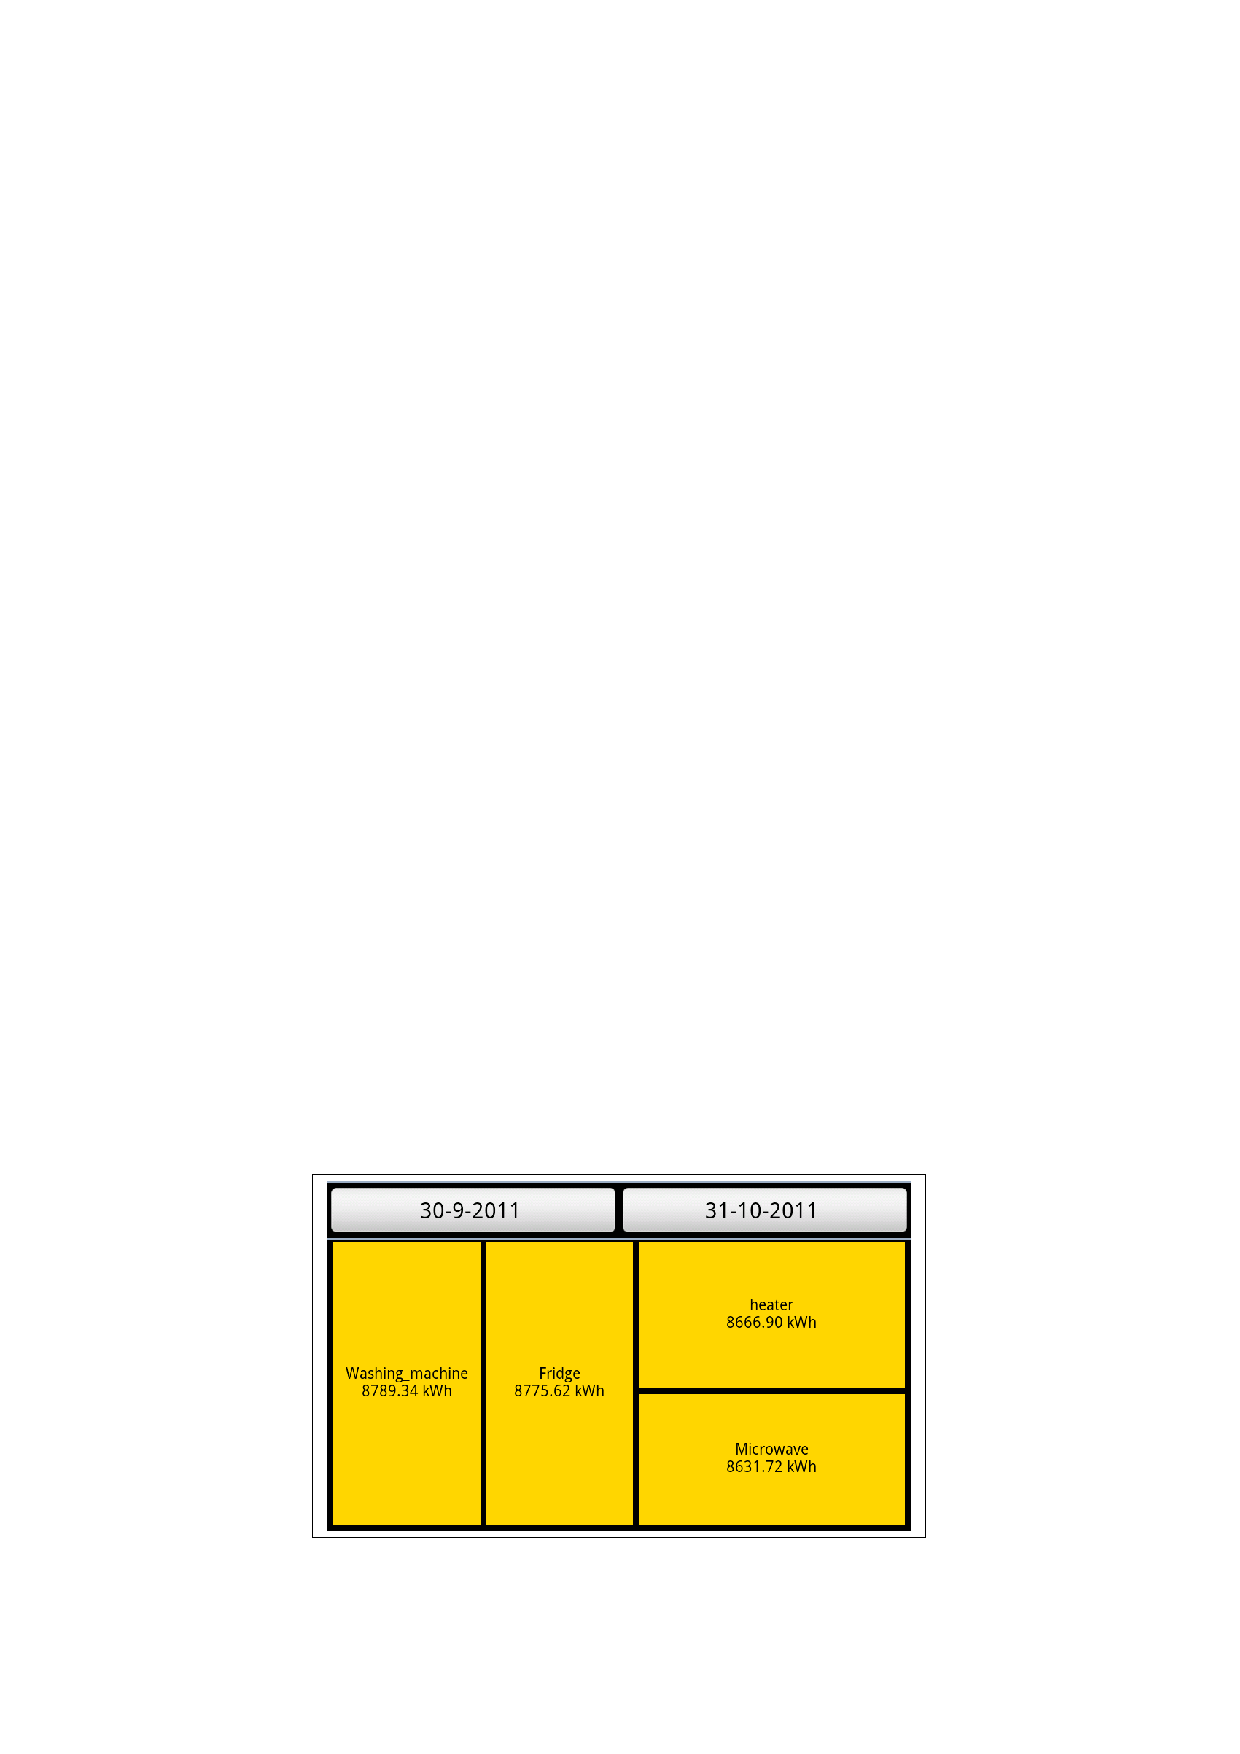
\includegraphics[scale=0.78]{images/mobile-treemap} 
\par\end{centering}

\caption{The treemap view, as shown by the Android application. Data returned
from meters, which have directly comparable units, can be displayed
in this view in order to get a quick overview of the energy consumption
relationship between meters or devices.\label{fig:treemap-android}}
\end{figure}


To give mobile users an opportunity to gather an insight into their
telemetry data, a mobile application for Android was developed as a client
for WattsApp. This mobile application provides a simple and intuitive way of 
viewing data (power consumption, water consumption, etc.) that is passed to 
it, as well as of modifying information related to meters that collect data. This
application has been made available in the Google Play store.

The WattsApp application uses Facebook credentials in order to authenticate
itself with the server that provides the data. It also uses a single
sign-on feature so that if the smartphone has a Facebook application
installed and the user is logged into it, signing into the WattsApp
happens automatically. Otherwise, when the application is launched
the first time, a Facebook login screen is presented to the user.
Once the user provides credentials and is successfully logged in,
appropriate permissions needed by the application (access to the e-mail
address of the user) must be accepted. After successful authentication
the application stores the Facebook access token, the user ID and
the time for which the token is valid since this data is used to support
the Single Sign-On feature.

\begin{figure}[t]
\begin{centering}
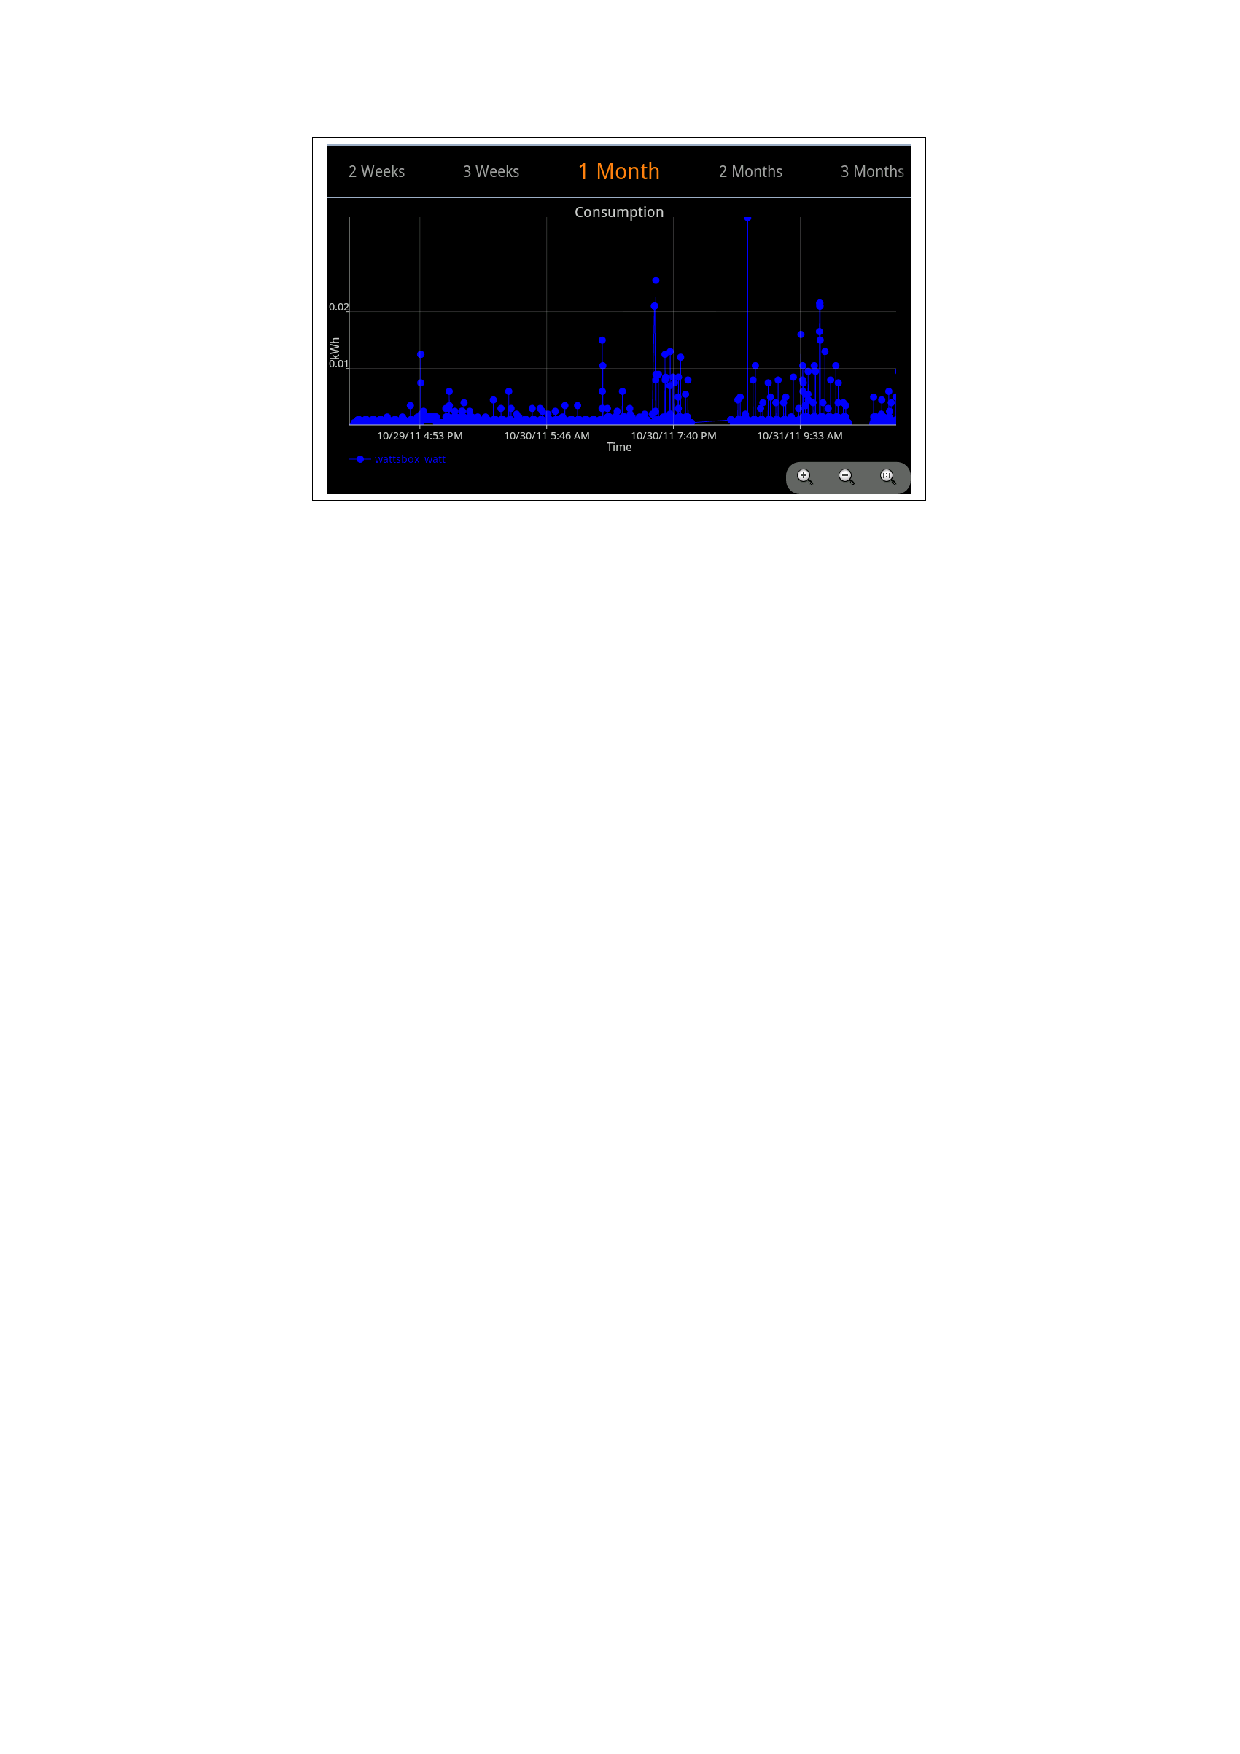
\includegraphics[scale=0.78]{images/mobile-graph} 
\par\end{centering}

\caption{The detailed graph mode, as shown by the Android application. Data
displayed in this view can provide deeper insights into the energy
consumption patterns.\label{fig:graph-android}}
\end{figure}

Authentication and permission levels are retrieved from the WattsApp
server, i.e. the gatekeeper at the cloud server, by supplying to it
the user ID for which the token was obtained. Since the WattsApp server
has access to the token and user ID information as well, a successful
match can be used to confirm the users' identity. Following this,
the WattsApp server looks up the list of collectors a user has access
to (including administrator privileges) and returns this data to the
mobile application. The user can filter the meters by their units
as well as the collectors which the meters are associated with. In
case a user has full read-write permissions on a particular meter,
an edit button is presented in front of the appropriate meter. Pressing
the edit button displays a meter configuration page, where the user
can rename a meter or manually set its new location.

%\vskip 1.37cm
%\pagebreak
 
A user may select multiple meters to display the data from
by selecting the check boxes next to each meter. Data from meters can
be displayed in two modes - Treemap or Graphical plot. In the Treemap mode
only the information obtained from the devices that measure comparable
data (i.e. has the same measurement units) can be viewed. The Treemap
display, shown in Figure \ref{fig:treemap-android}, is useful to
observe the relative relationship at a glance. For further insight,
the user can tap on meters in the Treemap display and choose to graph
these, as shown in Figure \ref{fig:graph-android}. The graphing capability
was added using the Achartengine API%
\footnote{http://www.achartengine.org/%
}, which is distributed under the Apache 2.0 license. The user can 
select the time period for which the data is plotted by either
using a calendar to pick the exact time frame, or using a rotating
picker that allow picking between pre-set options (e.g. one-month,
one-week, etc.).

One more feature WattsApp provides is the ability to search for the
collectors in the local network by the means of mDNS. Our original
intention was to use the jMDNS library%
\footnote{http://jmdns.sourceforge.net/%
} for this purpose, the most popular open-source mDNS Java solution.
However, when IPv6 was used, we faced difficulties with running it
on the Android devices. Therefore, we decided to make use of the standard
\verb=java.net= package in order to join the IPv6 multicast group
and listen to the advertisements sent out by the collectors on the
local network.


\section{Related Work}

The IETF EMAN working group is currently defining a set of MIB modules
for power and energy management of devices and for monitoring batteries.
While these MIB modules will provide a much more detailed approach
to monitor and manage so called energy objects, it was for us sufficient
to utilize the existing ENTITY-SENSOR-MIB \cite{rfc3433}.

The S0 interface \cite{iec62053-31} used by our meters is a very
simplistic interface since it only defines pulses and it does not
entail any data communication. As such, S0 is a very cheap solution
for small installations but lacks in providing further details about
what S0 pulses represent, nor is there information about quality aspects
of the power consumed. More advanced meters make use of the MODBUS
protocol \cite{iec61158}, which can run over serial lines but also
over TCP connections. MODBUS provides much more functionality but
also requires more logic inside of the meters, hence impacting the
price of the meters. Given our system design, we would interface MODBUS
devices, in particular MODBUS over TCP capable devices, directly with
the collector instead of using a wireless sensor mode between the meter and the collector.


\section{Conclusion}

Given the short time frame of just over one month to take WattsApp
from inception to completion, a fully working system capable of delivering
energy usage data to the user is a positive outcome. Adoption of the S0 interface ensures that WattsApp can be used to track utilities, beyond electricity, like gas and water as well. However, the ability to compare
data between different types, e.g. temperature and electricity consumption,
makes WattsApp an interesting tool suitable for demonstration of the
capabilities of the IoT. The successful integration
of multiple technologies within WattsApp, at a rapid pace, is proof
that enough tools exist to develop distributed applications using
IPv6 for all communication between the components.

Given the seeming popularity of S0 meters, we were surprised that digital interface circuitry for these was not easily available. The only products were USB interfaces, which worked with proprietary
data formats and applications. A lack of open and non-proprietary
interface devices prompted us to design our own S0 interface circuit.

Due to the short development time, certain design decisions made can be changed to improve user experience. For example, currently the gatekeeper acts as a broker for all data exchange between the user interfaces and collectors. However, removing the gatekeeper from the data-path could considerably improve latency issues.

It is also interesting to note that this student project has had over
1000 downloads of its mobile app, and we have recorded over 700 registered
users on our web application. This can possibly indicate a high interest
in such energy monitoring applications.

\bibliographystyle{IEEEtran}
\bibliography{wattsapp-paper}

\end{document}


